
\section{Half Wave Plate modulation}

\begin{itemize}
\item les HWP deviennent a la mode
\item les kids ont des constantes tres petites, donc on peut faire tourner vite
  : avantages...
\item ... mais signal parasite tres fort et donc besoin de le soustraire et de
  voir si il n'induit pas de non linearite sur la mesure du signal
\item simulations du HWPSS (beta): bien expliquer que ce qui compte c'est la
  subtraction of this template not the exact recovery of the input model
\item which constraints do we set on the HWPSS subtraction and potential
  improvement if we could use hundreds of KIDS rather than just fit it kid by kid
\item anticipate a bit on the achieved residual NL on the same planet as in the
  previous section.
\item simulate the sum of a template and pure weak signal and see the induced NL
  on the signal
\item comparison to NIKA(2)'s data... vs Simon's observatory perspectives
\end{itemize}

{\color{blue}
Modulation of the polarization by a rotating Half Wave Plate (HWP) like in
\nika\ and \nikad\ creates a background modulation equivalent to several tens to
hundreds of Jy at frequencies close to the HWP rotation harmonics
\citep{2017A&A...599A..34R}. After early tests by \todo{cite Hildebrand in the
  80's or so ?}, this kind of modulating device has been left aside for
\todo{20~TBC} years in the context of millimetric observations. With the
improvement of technologies it progressively came back in the landscape, in
particular with pioneering experiments like \emph{Maxipol}
\citep{2007ApJ...665...42J} and \emph{EBEX} \citep{2010SPIE.7741E..1CR}. It is
now more and more common and is considered as the leading option for future
satellite designs such as \emph{LiteBIRD} \todo{add ref}. Such a background must
be accounted for in the simulations.}

\begin{figure}
	\includegraphics[clip, angle=0, width=\columnwidth]{Figures/histos_epsilon.eps}
	\caption{histos epsilon}
	\label{fig:histos_epsilon}
\end{figure}
